\chapter{Generalidades del proyecto}

\section{Descripción de la empresa u organización y del puesto o área de trabajo}
Limón Almacenes Sociedad Anónima de Capital Variable es una entidad dedicada a la compra-venta, distribución y consignación de abarrotes en general con R.F.C. LAL920610L86 localizada en Carretera Alazán-Canoas S/N km 68-A, Colonia 10 de mayo, C.P. 92100, Tantoyuca, Veracruz, México. Por su parte, el Departamento de Sistemas tiene como finalidad dar soporte a cada una de las sucursales que conforman la empresa, así como la Bodega Matríz; en este departamento se desarrollan las actividades de Soporte de Equipo de Cómputo, Instalación y Mantenimiento de Redes, Administración de Base de Datos, Capacitación para el Personal y Desarrollo de Herramientas en la Plataforma Java para la Administración y Control de la Empresa, y Atención al Cliente.
\\
\\ La estructura organizacional de la entidad está conformada por el Consejo de Administración seguida de una Dirección General que se divide en 8 departamentos entre los cuales se localiza el Departamento de Sistemas que está integrado por el área de Soporte e Inventarios, figura \ref{organigrama}.

\begin{figure}[!h]
	\centering
	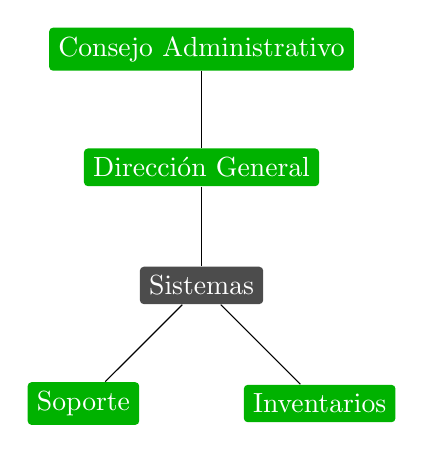
\begin{tikzpicture}[
	every node/.style={rectangle, text=white, rounded corners=0.05cm},
	grande/.style={fill=black!30!green},
	participacion/.style={fill=white!30!black}]
	\node[grande] {Consejo Administrativo}[sibling distance=6cm]
	child {
		node[grande] {Dirección General}
		child {
			node[participacion]{Sistemas}[sibling distance=3cm]
			child {
				node[grande] {Soporte}
			}
			child {
				node[grande] {Inventarios}
			}
		}
	};
	\end{tikzpicture}
	\caption{Organigrama específico de Limón Almacenes S.A. de C.V.}
	\label{organigrama}
\end{figure}

\section{Problemas a resolver}
Este proyecto surge para dar solución a los problemas que atañe a Limón Almacenes S.A. de C.V., en particular pretende resolver los siguientes puntos:

\begin{itemize}
	\item Reducción de costos en la adquisición de lectores de código de barras.
\end{itemize}

\section{Objetivo general, objetivos específicos y metas}
\subsection{Objetivo general}
Desarrollar una aplicación móvil, en dispositivos Android, que funja como un verificador de precios a los clientes de almacenes limón.
\subsection{Objetivos específicos}
\begin{itemize}
	\item Diseñar la interfaz de usuario.
	\item Codificar los diseños y la lógica de negocio.
	\item Realizar pruebas de caja negra y caja blanca.
\end{itemize}

\section{Justificación}
Los productos que oferta Limón Almacenes cuentan con su respectivo precio en los estantes correspondientes (Se dan casos en que no cuentan con él, sea por el deterioro de la etiqueta o que simplemente no cuente con ella). Y aunque los productos tengan su precio correspodiente, el cliente no tiene la seguridad suficiente para confiar en estos precios, por lo cual van al verificador de precios para corroborar que sea así.
\\
\\
Debido a la problemática identificada se plantea el desarrollo de una aplicación móvil en la que el cliente pueda verificar el precio del producto en su teléfono inteligente sin tener la necesidad de buscar en la sucursal un verificador de precios, agilizando el proceso de compra del mismo.